\chapter{Waveguides}
\label{sec:7_waveguides}

This chapter is dedicated to the question of how to guide light using optical fibers.
We begin by discussing why waveguides are necessary in long-distance communication before focusing on the main optical principles that allow us to confined light within optical fibers.
We conclude this chapter by looking at the basic construction of optical fibers and some of their basic types and properties.

\section{Brief history of guiding light}
\label{sec:7-1_history}

% EVEREST -> Everest
\begin{figure}[H]
    \centering
    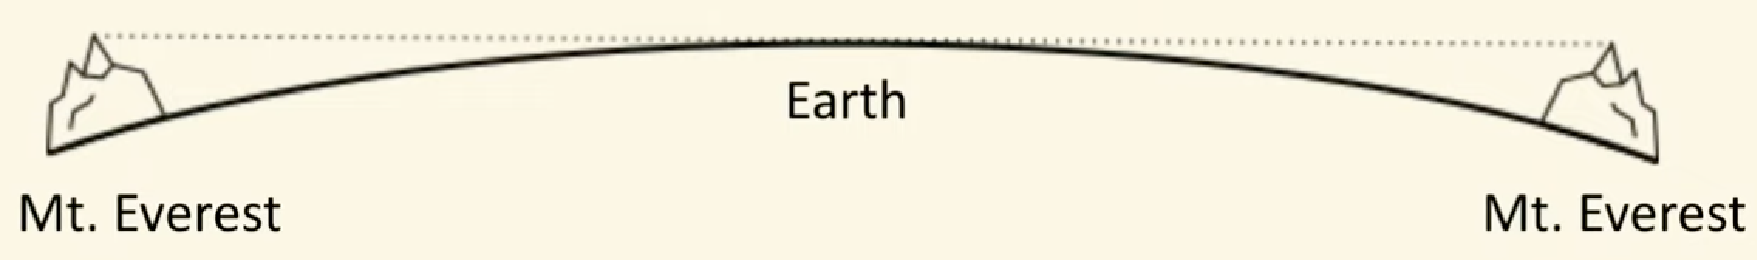
\includegraphics[width=0.9\textwidth]{lesson7/everest.pdf}
    \label{図: 1}
    \caption{The disadvantage of direct transmission of light.}
\end{figure}

Light is an excellent information carrier.
In previous chapters, we have focused mainly on light's speed and robustness to noise as the reasons that make it so suitable for communication.
We have not really discussed another important property of light, namely that is travels in \textit{\textbf{straight lines}}.
At first, this might seem like another advantage.
Coupled with light's speed and insensitivity to noise, it would seem that all we have to do is point at our intended target and light will carry our message to its destination unimpeded.
However, this is not quite true.
Due to the curvature of the Earth, the range of direct transmission is limited.
This range depends on the altitude at which the source of light as well as the receiver are found.
In order to increase the range, both need be placed as high as possible.

Let's perform a little thought experiment in order to get an intuition for the maximum distance the transmitter and receiver can be separated by before they lose direct line of sight due to the curvature of the Earth.
Consider placing the light source at the highest point on Earth, the top of Mount Everest at 8849 meters above sea level.
And let's say that there is another Mount Everest with the receiver placed at its top.
How far the two mountains be such that they are just able to maintain direct line of sight, assuming there are no obstacles between them?
With some basic trigonometry, the answer comes to a mere 672 kilometers.
And this is without worrying about absorption due to bad weather.

Being able to transmit light through a waveguide gets around some of these problems.
Weather conditions are no concern anymore.
Absorption is still an issue but not a fundamental obstacle as we will learn in Chapter \ref{sec:11_long-distance}.
Before learning how optical fibers work, it is worth at some brief history of guiding light.

One of the earliest 

Let's see how it all began with John Tyndall's experiment. In 1870, he took a big bucket, filled it with water, and created a small hole on one side of the bucket at the bottom. He noticed that sunlight that was going into the water was also exiting through this opening in the bucket. But to his surprise, the sunlight not only came out the hole, but also followed the trail that was being taken by the water itself. The sun's rays did not just exit the water bucket in a straight line, but they were being guided by the water itself. So this was one of the first examples of actual fiber, where light was being reflected inside the fiber and guided, and not traveling just in a straight line.

Here's a brief historical outline of the journey that fiber optics have taken. It all began in 1870 with John Tyndall's experiment. From that point on, people were slowly investigating fiber optics and how to guide light, particularly in glass, but it was only really in 1960 with the invention of the laser when people truly realized the potential of using laser light coupled to fiber optics. They spent a lot of effort in researching how to do that, and in 1966 people managed to couple lasers with fiber optics. This really sparked the first information revolution (and was rewarded with a Nobel Prize in Physics for it). Just to give you some idea how far we've come, in 1970 it was possible to transmit about one percent of the original light over a distance of one kilometer, meaning that if you put in light of some power at the beginning, after one kilometer, you only had one hundredth of the original signal remaining. Twenty years later in 1990, it was possible to transmit ninety six percent (96\%) of the original power over the same distance of one kilometer.

And where are we now? In 2021, well, let's have a look at the map of a submarine fiber optic cables. So you can see how many, many cables there are connecting the continents across the Pacific, across the Atlantic, also going from different continents to other continents like this (follow pointer), and this is only the map of the submarine cables. Even more cables go over land than under the ocean, so truly the fiber optic network is the nervous system of mankind, allowing us to communicate within milliseconds from one side of the Earth to the other.

Let's have a quick look at what we're going to talk about in this chapter. First, we're going to begin with two basic phenomena of how light behaves when it hits the interface of two materials. We're going to talk about reflection and refraction. These two are crucial for understanding how fiber optics works. Then we will talk about total internal reflection, where we're going to combine reflection and refraction and derive the condition for total internal reflection. Total internal reflection is what we have seen in Tyndall's experiment, where light was not escaping the water stream but it was being reflected and guided by the water stream. We will conclude by some basics of fiber optic cables, in particular how they are constructed and the differences between various types of optical fibers.


\section{Light at an interface}

Let's see what happens when light is trying to go from one medium into a different medium.  To make this quantitative, we need a way to describe light.  There are three major descriptions we can use, useful in different circumstances.  First, light can be viewed as a particle traveling in straight lines, basically like a ray (or vector). In order to describe that ray, all we need is \emph{geometric optics}. This is the easiest scenario. Geometric optics relies basically on the laws of trigonometry to describe how the path of light changes as it travels from one medium to the other.

If we are interested in the properties of light as a wave, such as we saw with the double-slit experiment, the next step up is to embrace that wave behavior.  The wave description holds whether it's coherent light as from a laser, or in the form of single photons. In order to describe laser light, particularly when it's traveling down very narrow fibers, we need Maxwell's equations and the full theory of electromagnetism. This description is a lot harder and we're not going to use it here~\footnote{Maxwell's equations are covered in the second module in this series, "From Classical to Quantum Light".  They use partial differential equations (PDEs), which we briefly introduce in that module, but we recommend taking a math class that covers PDEs if you can. The more you have worked with PDEs the easier Maxwell's equations will be.}.

Finally, the third description is quantum field theory, because light fundamentally is a quantum field. Surprisingly given the theme of of this book, we're not going to worry about this at all. We're only going to use geometric optics, so the most simple description because mainly we will consider the diameter of the fiber to be much larger than the wavelength of the light, so here $d$ is the diameter of the fiber and $\lambda$ (lambda) is the wavelength of light. To give you some ballpark of the numbers that we're going to consider, $d$ varies somewhere from 10 all the way up to 200 micrometers, whereas the wavelength of the light we are considering is around of the order of fifteen hundred nanometers (1500nm), in what is known as the near infrared band.

Let's see what happens when the light arrives at an interface of two media. We're going to consider one medium, usually the air, and then some denser medium, let's say that it's glass. The light ray is going to arrive at some angle, and this angle will always be measured with respect to the normal to the surface. So we're not going to talk about the angle of incidence as that angle (follow pointer) but the angle between the light ray and then this orthogonal normal line to the surface. So this is the angle of incidence, and we're going to denote it $\theta_i$ (theta i).

The light can actually reflect off the surface, as this (see pointer), at some angle which we're going to call $\theta_R$ ("theta capital R"), the angle of reflection, and also some portion of the light will get refracted, so it will travel into the medium at some angle $\theta_r$ ("theta small r"), the angle of refraction. Notice that all of these angles are defined with respect to the dotted line which is the normal to the surface, that's very important.

Often, some portion of the light is reflected, some portion of the light is transmitted into the other medium, getting refracted as it does so. In this case, we're saying that, for example, ninety percent of the light is refracted and enters the glass whereas ten percent gets reflected back. But, we're not going to be too interested in the relationship of how much gets reflected and how much gets refracted, we are more interested in the angles of reflection and angles of refraction. So what is the angle of reflection? Well, that's very simple. The angle of reflection is just the angle of incidence, so $\theta_i = \theta_R$. For example, if we keep increasing the angle of incidence, so we started with this light right here (follow pointer), but then we consider a different light ray, and then a different one, all with different angles of incidence, the corresponding angles of reflection are also increasing.

Now, let's talk about angle of refraction. This is going to be a little bit more complicated. As you can see from this image here, the angle of incidence and angle of refraction are different. So let's see how we can actually compute them, and for that, we need something called refractive index of a material.

Refractive index is defined as follows: we're going to denote it as $n$, and it's given as $c/v$, where $c$ is the speed of light in vacuum, and v is the speed of light in the medium. So really, what refractive index tells us is how much does the speed of light change in this new medium. For example, this refractive index of vacuum is just one. Why? Because in vacuum, the light travels with the same speed c, so $c$ over $c$ is equal to one. Air has a slightly larger refractive index, but for our purposes it's basically just one, so the speed of light does not change very much, it slows down a little bit but very very small amount. Glass on the other hand, has a refractive index of 1.46, so it means that the light travels 1.46 times slower in the glass than when we compare it with the speed of light in vacuum. And in diamond, it travels even slower by a factor of 2.42, which is the refractive index of diamond.

Let's get back to our example of light ray being incident on a surface.

We're going to denote the refractive index of the top medium as $n_i$. $i$ stands for anything that's incident onto the surface. $n_r$ is the refractive index of the material into which the light ray transmits and gets refracted. The angles follow this relationship (eq. on top right), so the sine of the incidence angle, divided by the speed of light in that medium, is equal to the sine of the refracted angle$\theta$R, over the speed of light in the new medium.

$n_i=c / v_i, n_r=c / v_r$

We can use this relationship between the refractive index and the speed of light in the medium, and we just substitute for $v_i$, and we substitute for $v_r$, and we obtain the following relationship: it's $n_i$ times sin(theta i), is equal to $n_r$ sin($\theta_r$). So the refractive index of the medium on top here ($n_i$), times the sine of the incidence angle $\theta_i$, is equal to the product of the refractive index of the new medium and times the sine of angle of refraction. This is known as \emph{Snell's law}\index{Snell's law}, and this law is very useful and we're going to use it extensively in this and following lessons.
\begin{equation}
\frac{\sin \theta_i}{v_i}=\frac{\sin \theta_r}{v_r}
\end{equation}

\begin{equation}
n_i \sin \theta_i=n_r \sin \theta_r
\end{equation}

\begin{equation}
\begin{gathered}
n_i \sin \theta_i=n_r \sin \theta_r \\
\frac{n_i}{n_r}=\frac{\sin \theta_r}{\sin \theta_i} \\
<1
\end{gathered}
\end{equation}

Before we do any computations, let's see what actually happens with the angles as light travels from, let's say a less dense medium into a more dense medium, which will give us the relationship $n_i < n_r$. For example, consider the example of light traveling in air and then trying to move into glass. Again, substituting into our Snell's law and rearranging a little bit, we've got $n_i$ over $n_r$, so we brought this $n_r$ on to the other side (LHS), and then we also divided by sine$\theta_i$, so we've got that the fraction of $n_i / n_r$, has to be equal to sine$\theta_r$ over sine$\theta_i$. And from our assumption that we are traveling from less dense medium into more dense medium, we can see that the fraction of the left-hand side is smaller than one. What this means that this fraction over here (RHS) also has to be smaller than one, and that's achieved when $\theta_r < \theta_i$, meaning that the angle of refraction is smaller than the angle of incidence. So we see that when light travels from a less dense medium into more dense medium, it bends towards the normal. 

What happens in the opposite scenario when we are traveling from a more dense medium into a less dense medium? Well, we can go through the same calculation again, but this time we assume that $n_i > n_r$, and we substitute it in. We see that the ratio on the left hand side of $n_i/n_r > 1$, therefore we conclude that the angle of refraction has to be larger than the angle of incidence, so if we are going from a more dense medium into a less dense medium, we are refracting away from the normal.


\section{Total internal reflection}


In the previous section, we saw that if light is incident on a surface and traveling from a more dense medium into a less dense medium, then it gets bent away from the normal axis. The angle of refraction is larger than the angle of incidence, $\theta_r > \theta_i$. Consider the scenario where we are increasing steadily the angle of incidence, and the refracted beam of light is being bent further and further away from the normal axis that's perpendicular to the surface of the material. So we can ask the question: is there such an angle of incidence where the refracted beam travels parallel to the surface to the interface between the two media? Meaning, we are looking for a scenario where the angle of refraction is ninety degrees, and yes, there is. So we are looking for this scenario (see slide), we have our incident beam hitting the interface between glass and air at such an angle such that the refracted beam travels at ninety degrees to the normal, or parallel to the surface between air and glass. Let's now compute this angle using Snell's law.  Replacing $\theta_i$ with $\theta_c$ to represent this critical angle,

\begin{equation}
\begin{aligned}
&n_i \sin \theta_i=n_r \sin \theta_r \\
&n_i \sin \theta_c=n_r \sin 90^{\circ} \\
&n_i \sin \theta_c=n_r \\
&\sin \theta_c=\frac{n_r}{n_i} \\
&\theta_c=\sin ^{-1}\left(\frac{n_r}{n_i}\right).
\end{aligned}
\end{equation}

%We have that the $n_i$, the refractive index of glass, times the sine of the angle of incidence, is equal to the refractive index of air $n_r$, times the sine of $\theta_r$, but we know that here we are looking for a scenario where the sine of $\theta_r$ is just sine of ninety degrees which is equal to one. So we have the following relationship (see pointer), and we have changed the subscript here on this $\theta$ to "$\theta_c$" which stands for "critical angle", because that's the critical angle where we obtain angle of refraction of ninety degrees. Now we can just rearrange to get sine of $\theta_c$, equal to as a simple fraction of $n_r / n_i$. In our case, here $n_r$ is the refractive index of air and $n_i$ is the refractive index of glass, and we can just take the arc sine ($\sin^{-1}$) to obtain this expression for the critical angle. 

When light is at this angle $\theta_c$, then after reaching the interface the light ray travels parallel to the surface. We  can also keep increasing the angle of incidence so that $\theta_i$ is larger than the critical angle $\theta_c$.  When $theta_i > \theta_c$, we get "total internal reflection", so the light ray comes in and gets totally reflected back to inside the glass. This is the case that we saw in the first section of this chapter, where the light in Tyndall's experiment was being internally reflected and guided by the stream of water.

Let's consider some numerical examples. We keep the refractive index of the outside medium, which for us is air, fixed. It's just 1.00028, which we can round to just $1$. If we consider different choices for the material of the fiber, with differences in refractive index of $n_i$, we can find the value of the critical angle beyond which total internal reflection can occur. If we plot the arcsin of the previous expression for the $\theta_c$, then we get the curve in Fig.~\ref{fig:critical-angle}. So we see that as we are increasing the density \rdv{is this literally g/cc, or some other definition?} of the material, we are decreasing the critical angle beyond which we get total internal reflection. For example, if we look at the interface of water and air, water has a refractive index of 1.33, and we obtain a critical angle of around fifty degrees. Glass is a little bit more dense than water, it has refractive index of 1.46 and the critical angle beyond which we get total internal reflection is a little bit smaller than the critical angle for water. For diamond, which has a very large refractive index of 2.42, then the angle is slightly over twenty degrees. So what does all this mean, that the critical angle is decreasing? Well, it means that in glass, if we want to obtain total internal reflection, then the angle of incidence has to be large, meaning that the angle between the surface interface between air and glass has to be quite small.  So, light that hits that interface at a very shallow angle will experience total internal reflection. Whereas in diamond, the light is confined more strongly. It can have a incident angle which is smaller than it is in glass, so even if light is incident on the surface at a much steeper angle, it still can get reflected and be contained and guided by the fiber.



\section{Optical fibers}

Let's have a look at the composition of a typical optical fiber.  Often, many fibers are bundled into a fiber-optic cable, but here we will look at an individual fiber.  The outermost layer is the \emph{jacket}, and this is to protect the inside components of the fiber. The next layer is the \emph{buffer}. The buffer is there also for protection, but it can also bundle multiple optical fibers.

Then we've got the \emph{cladding}, and this is the material that is responsible for reflecting light back and keeping it contained within the innermost layer, which is the \emph{core}. Cladding serves as a form of protection and prevents crosstalk, because if you have two cores next to each other, then light can easily escape to the other core, so you must separate them somehow and that's the purpose of the cladding. So these two components (cladding and core) are the ones that are optically important parts. Core is the one that carries the light signal and it has some refractive index$n_f$, "f" for fiber, whereas cladding has a smaller refractive index $n_c$, and that's the one that is responsible for reflecting light back into the core and keeping it constrained inside the fiber. There are two main types of fibers. One is the \emph{multimode fiber}\index{multimode fiber}, over here (see slide), so you can see that here the modes are represented by different spatial beams bouncing inside the fiber, \rdv{clearer definition of "mode" here would be good} whereas \emph{single-mode fibers}\index{single-more fiber} which are so narrow that there's only one mode permitted to travel inside the fiber.

Let's look at multimode fibers first. As we said, here all of these rays (see slide), they represent various modes of light traveling inside the fiber, and what's important for multimode fibers is the angle of acceptance. This is the angle represented by this gray cone over here, and if the light comes traveling inside the fiber within this light cone, then it will couple to the fiber and undergo many internal reflections inside the fiber, and basically be carried inside and be guided by the fiber. But, if the incident angle of the light is such that it is outside of the acceptance cone, then it will just hit the cladding and get refracted outside and get absorbed, so it will not be coupled to the fiber. So, let's apply Snell's law and actually calculate what is the maximum permissible permitted angle such that we couple to the fiber.

We have the following scenario: in here we actually have two interfaces. One interface is the usual between the fiber with refractive index $n_f$, and the cladding with refractive index $n_c$, but now we also have to consider the light coming into the fiber, so we also consider refractive index of some material that's outside of the fiber and we will denote it by $n_i$. And we've got these three angles (see slide). We are looking for the maximum $\theta$- maximum permitted angle, and if we multiply it by two, this is called the acceptance angle. And we want this angle to be such that when the light gets refracted into the fiber and then hits the cladding, it gets reflected completely and totally back into inside the fiber. So this angle, we set to $\theta_c$, which is the critical angle needed for total internal reflection. Using basic trigonometry, then we know that this angle of refraction at the surface of the fiber and whatever material is outside of the fiber has to be ninety degrees minus $\theta_c$.

And we all know from previous section that if we take the sine of this critical angle, so this angle over here (see pointer), it has to be equal to the ratio of the refractive indices of the cladding and the fiber, so sine $\theta_c$ is equal to $n_c$ over $n_f$.

Then we continue using our Snell's law, so at this interface between the fiber and the outside material (see pointer), we write that $n_i$, the refractive index of the outside material, times sine $\theta$ max, has to be equal to the refractive index of the fiber times sin(ninety degrees minus $\theta_c$), which is the angle of refraction over here measured with respect to the normal of the surface, which in this case is given by this horizontal dashed line.

We can simplify using a trigonometric identity.  sin(ninety degrees minus $\theta_c$) is just equal to the cosine of that angle $\theta_c$, and we can use another trigonometric identity where we use the fact that sine squared of an angle plus the cosine squared of the angle has to be equal to one. So cosine of $\theta_c$ is just equal to one minus sine squared $\theta_c$, the whole expression square rooted.

And using the expression that we have over here for the critical angle (see pointer), we can just substitute an expression for sine squared $\theta_c$, which is just $n_c$ squared over $n_f$ squared.

So finally, we have the following expression: multiplying this (see pointer) by $n_f$, we get that the $n_i$ times sine$\theta_{max}$, is equal to the square root of $n_f$ squared minus $n_c$ squared, and this gives us the "theta max", the maximum angle of acceptance and therefore also, the cone of acceptance.
\begin{equation}
\begin{aligned}
n_i \sin \theta_{\max } &=n_f \sin \left(90-\theta_c\right) \\
&=n_f \cos \theta_c \\
&=n_f\left(1-\sin ^2 \theta_c\right)^{1 / 2} \\
&=n_f\left(1-n_c^2 / n_f^2\right)^{1 / 2}
\end{aligned}
\end{equation}

\begin{equation}
n_i \sin \theta_{\max }=\left(n_f^2-n_c^2\right)^{1 / 2}
\end{equation}
And this number on the left hand side, this product of the refractive index times the max sine of the maximum acceptance angle, is known as numerical aperture, and the higher the numerical aperture is, the better we can couple to the fiber, meaning that this incident angle over here which we are calling$\theta_{max}$, is allowed to be larger.

So, what are some properties of multimode fibers? Well, we said that their diameter is much larger than the wavelength of the light, and typically they've got diameters larger than ten micrometers, and they can go up to something like two hundred micrometers. So we said, in order to describe their behavior, it is enough to consider light traveling as a particle traveling in straight lines, and using basic trigonometry, so we can use geometric optics which we have been doing so far in order to derive some useful properties of the multimode fiber.

Second, the light inside travels at different angles, meaning that it can carry multiple modes at the same time. Because the path lengths of the various light rays differ, we get \emph{mode dispersion}\index{mode dispersion}, which we will describe in more detail in a later lesson. Such a fiber, because of mode dispersion, is more suited for short distances, meaning inside office networks or campus networks. Also, it is relatively cheap to manufacture, mainly because it's quite thick. 

On the other hand, a single-mode fiber can carry only a single mode of light, so there's only one ray traveling in one direction like this (follow pointer). The core diameter for single-mode fiber is typically smaller than ten micrometers. Just to give you an idea how thin that is, the human hair is usually larger than twenty micrometers. There's a large variance, but the core diameter between twenty, and perhaps two hundred micrometers \rdv{wait, single-mode or multimode is 200um?  Above we said multimode. Also, this is about the third time we have said this in this chapter.}, so they're extremely extremely thin. Because they are so thin, it is no longer possible to describe light inside them using geometric optics. We have to resort to using electromagnetic theory and Maxwell's equations.

Because they are so thin, restricting the propagation of light to a single mode, there is no mode dispersion.  Mode dispersion changes the shape of the signal received at the far end, so the rate at which a signal can be changed while maintaining a clean signal at the receiver is determined by the amount of this dispersion. That is why single-mode fibers allow for very high rate of transfer of data, and therefore they are suitable for long distance communications. They have to be boosted by repeaters approximately every fifty kilometers, but we will see how that can be achieved in a later lesson. One disadvantage of single-mode fibers is that because they are so thin, they are quite expensive to produce.

Let's end this chapter with a small note: the first transatlantic fiber optic cable, which was called TAT-8, was laid in 1988 between Tuckerton, New Jersey, and then it traveled across the Atlantic and then split into the UK and France. The submarine cable was constructed at a cost of approximately 335 million US dollars, and it was retired in 2002. It was predicted that the bandwidth of this fiber optic cable would last for a long time and perhaps never be reached. The bandwidth was two hundred eighty megabits per second (280 Mbits/s), which can carry around forty thousand phone circuits simultaneously. This capacity was reached in eighteen months, necessitating the laying of more cables. This demonstrates how quickly how quickly we can consume available data bandwidth~\footnote{rdv finds it an interesting historical anecdote that one of Japan's first undersea cables came ashore in the seaside town of Kamakura, where he lives, in 1931.  At that time, the cable would have been copper rather than fiber.  It connected to Midway, Hawaii, then the continental U.S.  It was in use for around a dozen years.}

\newpage
\begin{exercises}
\exer{Consider the following quantum state:}
\begin{equation*}
\ket{\psi} = \frac{\sqrt{3}}{2}\ket{0} + \frac{1}{2}\ket{1}
\end{equation*}
\subexer{Find the probability of measuring a zero.}
\subexer{Find the probability of measuring a one.}


\end{exercises}

\newpage
\section*{Quiz}
  \addcontentsline{toc}{section}{Quiz}

\section*{Further reading Lessons 5-7}
  \addcontentsline{toc}{section}{Further reading Lessons 5-7}

Lesson 5

This Lesson discusses the various types of light depending on their coherence properties. Coherent light produced by lasers is crucially important from the perspective of communication. A good qualitative as well as quantitative introduction to lasers can be found in Chapter 1 of:

Orazio Svelto, Principles of Lasers, Springer, 2009.

A great discussion of lasing behaviour from the perspective of a mathematician (but still explained very intuitively) is in Chapter 3 of the classic:

Steven H. Strogatz, Nonlinear Dynamics and Chaos: With Applications to Physics, Biology, Chemistry, and Engineering, CRC Press, 2000.

Lesson 6

Two great optics textbooks for this Block as well as the following ones are:

Eugene Hecht, Optics, Pearson, 2015.
Grant R. Fowles, Introduction to Modern Optics, Dover Publications, 1989.
Bahaa E. A. Saleh, Malvin C. Twitch, Fundamentals of Photonics, Wiley-Interscience, 2007.

These books focus on wave and geometric optics and provide a good foundation for transitioning to quantum optics which we will do later.

Interference is an extremely important concept we encourage you to read and understand the discussion in Chapter 1 in:

Richard P. Feynman, Robert P. Leighton, Matthew Sands, The Feynman Lectures on Physics, Vol. 3, Addison Wesley, 1971.

Lesson 7

This Lesson relies mainly on the geometric description of light propagation. Section 4.3 and Section 5.6 of Hecht’s textbook contain great discussion of reflection and propagation in optical fibers, respectively.
